\chapter{Using the Library}
\label{chap:echo}

This chapter explores using the C++ library designed and developed in the previous chapters to implement an
audio plugin that can be used by audio host applications. This is an ideal usecase for the library, as audio
plugins are often implemented in C++, and follow a similar structure to the signal processors introduced in
\autoref{chap:blocks}, i.e. are defined by a number of input/output channels, and evaluated on buffers of
data passed in one at a time.

\section{The Effect}

The example developed in this chapter is a simple echo audio effect, i.e. a plugin that continuously repeats
its input with some delay, where each echo gets quieter and looses "brightness", i.e. the high frequency
components of the signal. Echos were introduced in the 1950s, and have become a staple of music production,
being used especially for vocals and guitars. The first analog echos were based on a tape loop, where the
input audio was continuously written and then read back. The continuous repetitions provided by an echo are
achieved using a feedback loop, meaning the output of the echo is sent back into the input, but with reduced
gain and/or other processing applied.

The echo effect designed here is a simple, but fully featured one. It has a variable delay time, feedback
gain control, and a simple low-pass filter in the feedback loop to gradually remove more and more high
frequencies from the repeated signal. Lastly it has a dry/wet mix control, to mix the original (dry) signal
with the output (wet) signal of the effect. The block diagram for the effect can be seen in
\autoref{fig:echoblock}, and the following sections will go through this block diagram one part at a time.

\begin{figure}
  \centering
  \includestandalone[width=\textwidth]{Pictures/block_echo}
  \caption{Block diagram of the echo effect.}
  \label{fig:echoblock}
\end{figure}

\subsection{Controls}
The effect has 4 control variables, which are exposed through LV2, and controlled by the UI generated by the
plugin host. In code, these are represented as \cpp{float} variables, which can be used in the EDA
expression by wrapping them in a \Block{ref} block (see \autoref{sec:eda_lit_and_ref}).

\begin{cppcodenl}
  float filter_a = 0.9;
  float time_samples = 11025;
  float feedback = 1.0;
  float dry_wet_mix = 0.5;
\end{cppcodenl}

The meaning of the individual controls will be explained where they are used in the following sections.

\subsection{Filter}

Echoes often include a low-pass filter in their feedback loop, meaning each repetition of the echo will not
only be quieter, but also proportionally lose more high frequencies than low. This seems most natural to the
human ear, since low frequencies travel further, and will thus be louder when a sound returns as an echo.

\begin{wrapfigure}[13]{r}{0.45\textwidth}
  \centering
  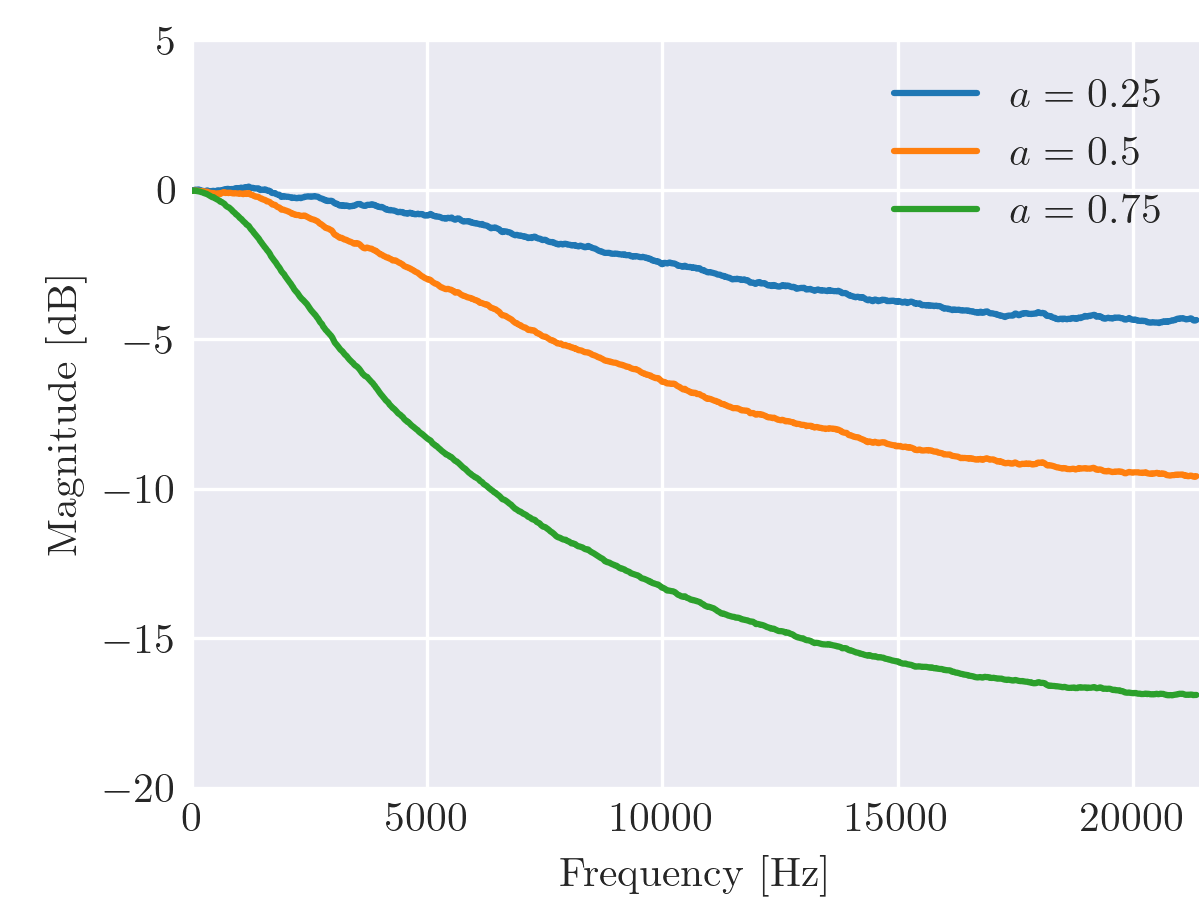
\includegraphics[width=0.45\textwidth]{Pictures/echo_filter_resp.png}
  \caption{Frequency response of the single-pole IIR filter used in the echo effect at different values of the
    $a$ parameter.}
  \label{fig:echo_filter_resp}
\end{wrapfigure}
% 
The low-pass filter used in this echo is the simplest DSP filter possible, a single-pole Infinite Impulse
Response filter. It can be understood as a weighted average between the input, and the previous output, i.e
its signal processor can be written as follows:
\begin{align*}
  \SigP{Filter}(a, s) & = y                                           \\
  y(-1)               & = 0                                           \\
  y(t)                & = (1 - a(t)) \cdot s(t) + a(t) \cdot y(t - 1) \\
  a(t)                & \in [0; 1]                                    \\
\end{align*}
% 
Here, $s$ is the audio input signal, and $a$ is a signal used to control
the weighting between the input and previous output, with higher values meaning high frequencies are more
suppressed. For an illustration of this parameter, see \autoref{fig:echo_filter_resp}, which plots the magnitude of
frequencies at a selection of values for $a$.

This particular filter is chosen mainly for the simplicity of its implementation, but it also fits the
purpose well, and results in a quite nice effect.

The EDA implementation of the filter follows from the relevant (green) part of the block diagram in
\autoref{fig:echoblock}, and can be written as such:

\begin{cppcodenl}
  ABlock<2, 1> auto const filter = (_ << (_, _), _) | (((_ * _) + ((1 - _) * _)) % _);
\end{cppcodenl}

Notably, this implementation uses the \Recursive block (\cpp[escapeinside=??]{?\%?}) to pass the result of the
previous iteration back into the filter. It also uses the \Split block (\cpp{<<}) to send
$a$ to both parts of the expression. By passing $a$ as a signal, this
filter becomes easily reusable, and could be included in a library of standard components.

\subsection{Echo}

This (blue) part of the block diagram contains the feedback loop and the delay, which perform the main work
of the effect. It is once again a recursive algorithm, meaning part of its input is its previous output.
Specifically, the output is passed through the filter discussed previously, multiplied by the feedback gain
control, and summed with the new input, to then be delayed by the specified echo time.

This block uses three control variables: \cpp{feedback}, which controls the feedback gain, \cpp{time_samples} which sets the delay time in
number of samples, and \cpp{filter_a} which is the $a$ control passed to the
filter. The signal processor for this part is % 
\begin{align*}
  \SigP{Echo}(s)(t)       & = x(t)                                                     \\
  \forall t < 0 : x(t)    & = 0                                                        \\
  \forall t \geq 0 : x(t) & = \SigP{Filter}(x')(t-time\_samples) \cdot feedback + s(t) \\
  x'(t)                   & =x(t-1)                                                    \\
  feedback                & \in [0; 1]
\end{align*}

Implemented in EDA, the code looks as follows: % 
\begin{cppcodenl}
  ABlock<1, 1> auto const echo = (plus | delay(ref(time_samples))) % (filter(ref(filter_a)) * ref(feedback));
\end{cppcodenl}

This uses the \Block{delay} block introduced in \autoref{sec:block_delay} to get the variable time
delay, and partial function application (see \autoref{sec:eda_partial_application}) to pass control signals with a nicer
syntax.

\subsection{Process}

Lastly, the outermost (red) part of the block diagram in \autoref{fig:echoblock} contains the dry/wet mix, to
mix between the unprocessed (dry) and processed(wet) signal. This is a very common control to have on all
kinds of audio effects, as it (together with the feedback gain control) is an easy way to get
\emph{more} or \emph{less} of the effect. The signal processor here is quite simple:
\begin{align*}
  \SigP{Process}(s)(t) & = mix \cdot \SigP{Echo}(s)(t) + (1 - mix) \cdot s(t) \\
  mix                  & \in [0; 1]
\end{align*}

The EDA implementation splits the input signal to both sides of a \cpp{+} operation, with the
one side passing through the \cpp{echo} block defined earlier, and one through the identity block \cpp{_}, with both sides multiplied by the appropriate mix
factor:

\begin{cppcodenl}
  ABlock<1, 1> auto const process = _ << (echo * ref(dry_wet_mix)) + (_ * (1 - ref(dry_wet_mix)));
\end{cppcodenl}

\section{Comparison with FAUST}

This example is a good opportunity to compare the EDA code to equivalent FAUST code. Here is the full EDA
program declaration from the previous section:

\begin{cppcodenl}
  auto filter = (_ << (_, _), _) | (((_ * _, (1 - _) * _) | plus) % _);
  auto echo = (plus | delay(ref(time_samples))) % (filter(ref(filter_a)) * ref(feedback));
  auto process = _ << (echo * ref(dry_wet_mix)) + (_ * (1 - ref(dry_wet_mix)));
\end{cppcodenl}

And to compare, the equivalent code in FAUST:

\begin{minted}[linenos=false]{haskell}
filter(a, x) = (((a * _, (1 - a) * x) : + ) ~ _);
echo = (+ : @(time_samples)) ~ (filter(filter_a) * feedback);
process = _ <: (echo * dry_wet_mix) + (_ * (1 - dry_wet_mix));
\end{minted}

A few syntactical differences can be seen. Setting aside the obvious \cpp{auto} prefix and
difference in operators, the main difference is FAUSTs support for function declaration syntax, which makes
the \cpp{filter} declaration a bit simpler to read. Mostly however, the differences are small, and
more work could be done to improve the syntax of EDA even further, where even something similar to fausts
function declarations should be possible.

\section{The Plugin}
\label{sec:echo_plugin}

The framework chosen to implement the echo plugin is LV2\footnote{\url{https://lv2plug.in}}, an open standard for audio
plugins, supported by applications such as Audacity\footnote{\url{https://www.audacityteam.org/}}, Ardour\footnote{\url{https://ardour.org/}} and
REAPER\footnote{\url{https://www.reaper.fm/}}. LV2 is similar to the more widely used alternatives such as
VST\footnote{\url{https://www.steinberg.net/en/company/technologies/vst3.html}} and AU\footnote{\url{https://developer.apple.com/documentation/audiounit}}, and is chosen here only for practical reasons, such
as better linux support and availability in Audacity, which provides useful analysis tools for scientific
purposes, such as the frequency spectrum analyzer used to generate \autoref{fig:echo_filter_resp} and similar plots
in \autoref{chap:multirate}.

An LV2 plugin consists of data definition files in the \emph{turtle} specification language, and
implementation in C/C++. For the EDA plugins, I wrote a small wrapper to write plugins as a C++ class instead
(see the appendix, page \pageref{codefile:example/lv2.hpp}), but it follows the structure of the C API closely.

The C++ code that implements the echo plugin can be seen in \autoref{lst:echo_lv2}. It consists of three
functions, that each are provided to the LV2 framework.

\begin{description}
  \item [\cpp{connect_port}] is called by the framework to provide pointers to the data ports. The four control
        are single values, and the two audio port pointers are arrays. All will be updated with values before each
        call to \cpp{run}.
  \item [\cpp{activate}] is called after all ports have been connected, before the first call to \cpp{run}, and in it
        the EDA blocks and evaluator are constructed. The evaluator is stored in a \cpp{DynEvaluator} a
        type-erasing wrapper for evaluators (see the appendix, page \pageref{code:dyn_eval}). Since the control ports
        are pointers to float values, they can be used directly with the \Block{ref} block.
  \item [\cpp{run}] is called to process incoming audio data. Its single parameter \cpp{n_samples} is the number of
        samples available in the audio port arrays given earlier, so the implementation is a simple loop through and
        call to the evaluator constructed in \cpp{activate}.
\end{description}

This implementation, along with a metadata file (see the appendix, page \pageref{codefile:example/echo/metadata.ttl}), defines the
plugin which is distributed as a folder containing the shared object binary and metadata. When installed on
the system, these can be used from a host program that supports LV2, such as Audacity, which will then
provide a UI for the controls. The UI generated for this effect by audacity can be seen in
\autoref{fig:echo_ui}.

\begin{figure}
  \centering
  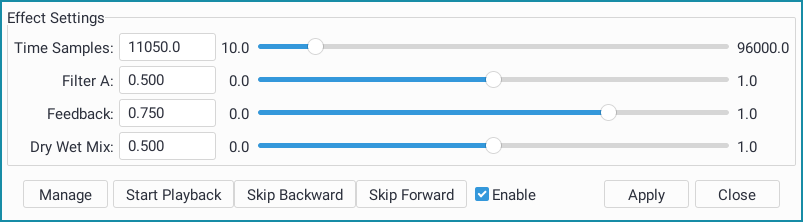
\includegraphics[width=\linewidth]{Pictures/echo_ui}
  \caption{The UI of the Echo plugin as displayed in Audacity.}
  \label{fig:echo_ui}
\end{figure}

\begin{listing}
  \begin{cppcodenl}
  struct Echo final : LV2Plugin {
    Echo() = default;

    void connect_port(uint32_t port, float* data) override
    {
      switch (port) {
        case 0: time_samples = data; break;
        case 1: filter_a = data; break;
        case 2: feedback = data; break;
        case 3: dry_wet_mix = data; break;
        case 4: input_port = data; break;
        case 5: output_port = data; break;
      }
    };

    void activate() override
    {
      ABlock<2, 1> auto const filter = (_ << (_, _), _) | (((_ * _, (1 - _) * _) | plus) % _);
      ABlock<1, 1> auto const echo = (plus | delay(ref(*time_samples))) % (filter(ref(*filter_a)) * ref(*feedback));
      ABlock<1, 1> auto const process = _ << (echo * ref(*dry_wet_mix)) + (_ * (1 - ref(*dry_wet_mix)));
      eval = make_evaluator(process);
    }

    void run(uint32_t n_samples) override
    {
      for (int i = 0; i < n_samples; i++) {
        output_port[i] = eval(input_port[i]);
      }
    }
    
  private:
    DynEvaluator<1, 1> eval;

    float* time_samples = nullptr;
    float* filter_a = nullptr;
    float* feedback = nullptr;
    float* dry_wet_mix = nullptr;
    
    float* input_port = nullptr;
    float* output_port = nullptr;
  };
  \end{cppcodenl}
  \caption{Implementation of Echo LV2 plugin}
  \label{lst:echo_lv2}
\end{listing}

\section{Performance Testing}

Only very minimal performance testing of the library has been done, and only of this single example program.
The performance was compared to an equivalent handwritten C++ program, by measuring 1000 iterations of
processing buffers of 1024 samples each. The code for this benchmark can be seen in the appendix, page
\pageref{codefile:tests/benchmarks.cpp}.

\begin{table}[H]
  \centering
  \begin{tabular}{|l|r|}
    \hline
    Program             & Average time pr. iteration \\
    \hline\hline
    Handwritten C++     & \SI{11.198}{\micro\second} \\
    % \hline
    EDA                 & \SI{16.770}{\micro\second} \\
    \hline\hline
    Relative Difference & +49.7\%                    \\
    \hline
  \end{tabular}
\end{table}

As a simple benchmark, this shows a performance penalty of roughly 50\%, which is very promising for the
completely unoptimized version of the library. It seems highly likely from this that some of the
optimizations mentioned in \autoref{sec:eda_conc} could reduce this number a lot, but of course more
measurements would need to be done in tandem with optimizations.

\section{Conclusion}

By showing a small EDA program and real-life usecase for the library, this chapter has illustrated the merits
of the library. I also compared the EDA implementation to an equivalent FAUST program, showing the minor
differences in syntax. To further explore the library in practical usage, more examples and testing should be
done, leading to further development and optimization of the library. However, even as presented in this
project, the library can clearly be used to implement at least semi-complex DSP algorithms and integrate them
in existing systems, with acceptable performance.
